\documentclass[11pt]{article}
\usepackage[margin=1in]{geometry}
\usepackage[T1]{fontenc}
\usepackage{lmodern}
\usepackage{amsmath,amssymb}
\usepackage{booktabs}
\usepackage{graphicx}
\usepackage{xcolor}
\usepackage[numbers,sort&compress]{natbib}
\usepackage[colorlinks=true,linkcolor=blue!50!black,citecolor=blue!50!black,urlcolor=blue!50!black]{hyperref}
\usepackage{caption}
\captionsetup{font=small,labelfont=bf}
\graphicspath{{../results/eic/}{../results/}}
\newcommand{\ci}[2]{\,[#1,\,#2]}
\newcommand{\Cov}{\mathrm{Cov}}

\title{Does Training Against Debate Reward Honesty?\\ Empirical Incentive Compatibility of Oversight Protocols
on Conceptual Reasoning}
\author{Abhimanyu Pallavi Sudhir}
\date{November 2026}

\begin{document}
\maketitle

\begin{abstract}
Scalable-oversight protocols such as debate are meant to be trained against: their value lies in making honesty
the policy that earns the most reward. Yet nearly all empirical work evaluates them by the judge's accuracy at
inference time, which a protocol that is useless to train against can score well on when today's models are
friendly. We instead measure \emph{empirical incentive compatibility} (EIC): the covariance between a protocol's
reward and the ground-truth honesty of the behaviour it rewards, over agent behaviours drawn by a \emph{sampler}.
That covariance is the first-order effect of reward optimization on honesty. We compare five protocols
(consultancy, sequential and simultaneous debate, recursive debate, prover-estimator debate) with three weak judges
on 927 conceptual-reasoning questions selected so that the agents know the answer and the judges do not, under
four samplers of increasing optimization pressure: instructed honest and dishonest arguments (ASD), the same with
only the arguments that actually lie, best-of-$n$ selection against the judge's reward, and prompt optimization by
a frontier model searching separately for the best honest and the best deceptive strategy. Instructed liars make
every protocol except prover-estimator look incentive compatible. Under optimization the picture splits: optimized
deception erases consultancy's incentive to be honest (held-out ASD $-0.24$, honesty wins on half the items),
deepens prover-estimator's deficit ($-0.37$), and shrinks but does not erase debate's ($+0.37$ sequential,
$+0.69$ simultaneous) and recursive debate's ($+0.09$). The cheap sampler only partly predicts the optimized one
(Spearman $0.40$ across protocol--judge cells). EIC rises steeply with judge capability (in debate, honesty
wins on 58--61\% of items with Llama-3.1-8B and 90--92\% with gpt-4.1) and, unlike accuracy, stays high for
judges that already know the answer. Prompted liars that refuse to lie, common among safety-trained models,
inflate a model's EIC from at most $+0.6$ to as much as $+4.0$.
\end{abstract}

\section{Introduction}

Debate \citep{irving2018debate} and its relatives are proposed as training methods: if a weak judge rewards
whichever agent argues better, and lies are harder to defend than truths, then optimizing agents against the judge
should make them honest. Empirical work on debate \citep{michael2023debate,khan2024debating,kenton2024scalable,
arnesen2024training} has nonetheless mostly reported the judge's accuracy at inference time. Accuracy and incentives
can come apart: a judge that simply believes the agent is accurate when the agent happens to be honest, and
useless to train against.

We study the incentive directly. For each episode of a protocol, every trained agent has two scores: the reward $u$
the protocol pays it (what training would optimize) and a ground-truth value $v$ of its behaviour, here $v = 1$ if
it argued the true answer and $0$ if it argued a false one. Training on $u$ moves an agent's policy $\pi$ in the
direction
\begin{equation}
\frac{d}{d\beta}\,\mathbb{E}_{\pi_\beta}[v] = \Cov_{\pi_\beta}(u, v), \qquad \pi_\beta \propto \pi_0\,e^{\beta u},
\label{eq:cov}
\end{equation}
the exact derivative along the KL-regularized optimization path. So the covariance between reward and honesty,
taken over the behaviours an optimizer could reach, is a cheap proxy for what training would do; its sign along the
path says whether the protocol is being Goodharted. Which behaviours it is taken over is set by a
\emph{sampler}. The agent score difference (ASD) of \citet{pallavisudhir2025asd} is the simplest: instruct the agent
to argue each side. Best-of-$n$ over sampled behaviour \citep{beirami2024theoretical} and prompt optimization
\citep{yang2023opro,agrawal2025gepa} reach further.

\paragraph{Contributions.}
\begin{itemize}
\item EIC estimates for five protocols under four samplers of increasing optimization pressure, on a
conceptual-reasoning benchmark with a 54-point gap between agents and judges, with selection and evaluation on
independent judge samples throughout (\S\ref{sec:samplers}--\ref{sec:po}).
\item A comparison of samplers: does the cheap instructed sampler rank protocols as optimization does
(\S\ref{sec:agreement})?
\item EIC across five judges of increasing capability on the same debates, and its dissociation from accuracy
(\S\ref{sec:judges}).
\item The refusal confound: models that will not lie make every protocol look incentive compatible
(\S\ref{sec:tournament}); and two hazards for anyone optimizing against LLM judges (\S\ref{sec:hazards}).
\end{itemize}

\section{Empirical incentive compatibility}\label{sec:eic}

\paragraph{Estimators.} With $v \in \{0, 1\}$, $\Cov(u, v)/\mathrm{Var}(v)$ is the difference of mean rewards
between honest and dishonest behaviour: the \textbf{ASD}, in the protocol's reward units (log score of the judge's
probability on the agent's answer for consultancy and debate; the judge's probability for recursive debate; the
prover's payoff for prover-estimator). We compute it per item and average over items. Because reward units differ
across protocols and inflate with confident judges, we also report \textbf{concordance}, the share of items on
which honesty earns more (0.5 = no incentive), and, where per-episode rewards exist, $r = \mathrm{corr}(u, v)$, the
normalized covariance. All intervals are 95\% percentile bootstraps over items.

\paragraph{Samplers.}
\begin{itemize}
\item \textbf{Instructed (ASD).} The agent is told to argue the true answer, then a false one (3 samples each).
\item \textbf{Committed liars.} The same, keeping only samples whose liars an auditor (gpt-5; agreement with Claude
Sonnet~5 $\kappa = 0.76$) found committed to the lie. A ``liar'' that concedes is not the dishonest behaviour
training could reach; this sampler targets effective lies.
\item \textbf{Best-of-$n$.} The agent's own behaviour re-weighted toward high reward: exactly over pools of 16
candidate arguments per decision for one-round protocols, and by keeping the best of $n$ candidates for every
speech of three-round protocols (a preview judge scores each candidate). Either only the liar is optimized, or both
sides are. A variant lets the agent choose which side to argue.
\item \textbf{Prompt optimization.} An optimizer (Claude Opus~5.5) that knows the protocol's rules and rewards
writes system-prompt strategies for the agent, in two separate searches per protocol and judge: one for the agent
assigned the true answer under an \emph{honest} directive, one for the agent assigned a false answer under a
\emph{deceptive} directive (``win anyway''). Each search runs five rounds of four candidates (GEPA-style reflection on
the best strategy's transcripts) on 36 training items. EIC is the ASD between the best honest and the best
deceptive strategy, both chosen on training reward and scored on 80 disjoint held-out items, after each round.
\end{itemize}
Every sampler that selects on the judge's reward is scored on an \emph{independent} judge sample: two samples of the
same judge on the same argument correlate only $r \approx 0.2$ within an item, so in-sample selection mostly
selects noise (\S\ref{sec:hazards}).

\section{Setup}\label{sec:setup}

\paragraph{Items.} 927 binary questions from 31 families of a conceptual-reasoning testbed (decision theory:
Newcomb, smoking lesion, twin prisoner's dilemma, Sleeping Beauty, Parfit's hitchhiker; social choice; number
theory; reward-hacking gridworlds; LLM auctions), selected from 3{,}437 because both agent models answer them
correctly on 2 of 2 samples while three weak judges are right on at most 60\% of 9 samples. On fresh samples the
agents are right 96--99\% of the time and the judges 41--46\%, below chance: the judges hold confident wrong
intuitions.

\paragraph{Models and protocols.} Agents: gpt-5-mini (medium reasoning effort; the main agent throughout) and Claude
Sonnet~4.5. Weak judges: gpt-4o-mini, Llama-3.1-8B-Instruct, Gemma-3-12B-it, each reasoning before stating
probabilities. Protocols, all with 200-word messages: consultancy (3 rounds, the judge questions the consultant);
debate (3 rounds, sequential or simultaneous); recursive debate (depth 2, width 3); prover-estimator debate (depth
2, width 3, $\rho = 2$; \citet{browncohen2025prover}). Debate seats are balanced across items.

\section{Instructed samplers}\label{sec:samplers}

\begin{table}[t]
\centering\small
\caption{EIC under the instructed samplers (gpt-5-mini agents, 3 weak judges pooled, 927 items). ASD in each
protocol's reward units.}
\label{tab:instructed}
\setlength{\tabcolsep}{4pt}\footnotesize
\begin{tabular}{lcccccc}
\toprule
& \multicolumn{3}{c}{instructed (ASD)} & \multicolumn{3}{c}{committed liars only} \\
\cmidrule(lr){2-4}\cmidrule(lr){5-7}
protocol & ASD & conc. & $r$ & ASD & conc. & $r$ \\
\midrule
consultancy & $+0.38$\ci{+0.29}{+0.47} & 0.61 & $+0.09$ & $+0.21$\ci{+0.12}{+0.31} & 0.55 & $+0.04$ \\
debate, sequential & $+0.74$\ci{+0.66}{+0.82} & 0.69 & $+0.18$ & $+0.56$\ci{+0.48}{+0.64} & 0.65 & $+0.14$ \\
debate, simultaneous & $+0.79$\ci{+0.70}{+0.87} & 0.72 & $+0.19$ & $+0.57$\ci{+0.48}{+0.65} & 0.68 & $+0.14$ \\
recursive debate & $+0.10$\ci{+0.08}{+0.11} & 0.64 & $+0.14$ & $+0.10$\ci{+0.08}{+0.12} & 0.62 & $+0.12$ \\
prover-estimator & $-0.13$\ci{-0.15}{-0.11} & 0.35 & $-0.14$ & $-0.23$\ci{-0.26}{-0.20} & 0.27 & $-0.26$ \\
\bottomrule
\end{tabular}
\end{table}

Under instructed arguments every protocol except prover-estimator pays more for honesty
(Table~\ref{tab:instructed}). Keeping only committed liars lowers every protocol's EIC (consultancy's by almost
half) but changes no sign and barely changes the ranking. Prover-estimator debate pays a prover more for defending
the false answer on two-thirds of items: without a coherent estimator its subclaim pricing rewards lying.
Figure~\ref{fig:heatmap} shows the same pattern for each judge; consultancy under Llama-3.1-8B is already negative
(instructed ASD $-0.26$\ci{-0.41}{-0.12}).

\begin{figure}[t]
\centering
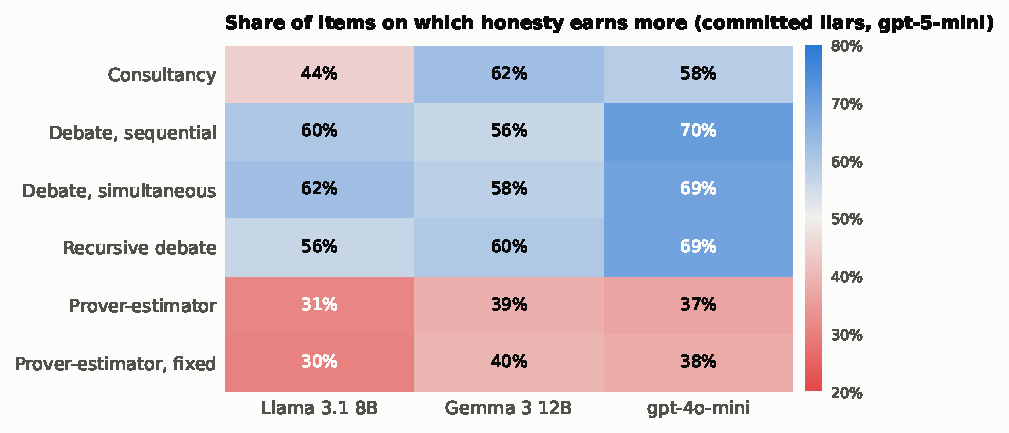
\includegraphics[width=0.62\linewidth]{fig7_concordance_heatmap_paper.pdf}
\caption{Share of items on which honesty earns more, per protocol and judge (committed liars, gpt-5-mini).}
\label{fig:heatmap}
\end{figure}

\section{Optimization pressure}\label{sec:bon}

\begin{figure}[t]
\centering
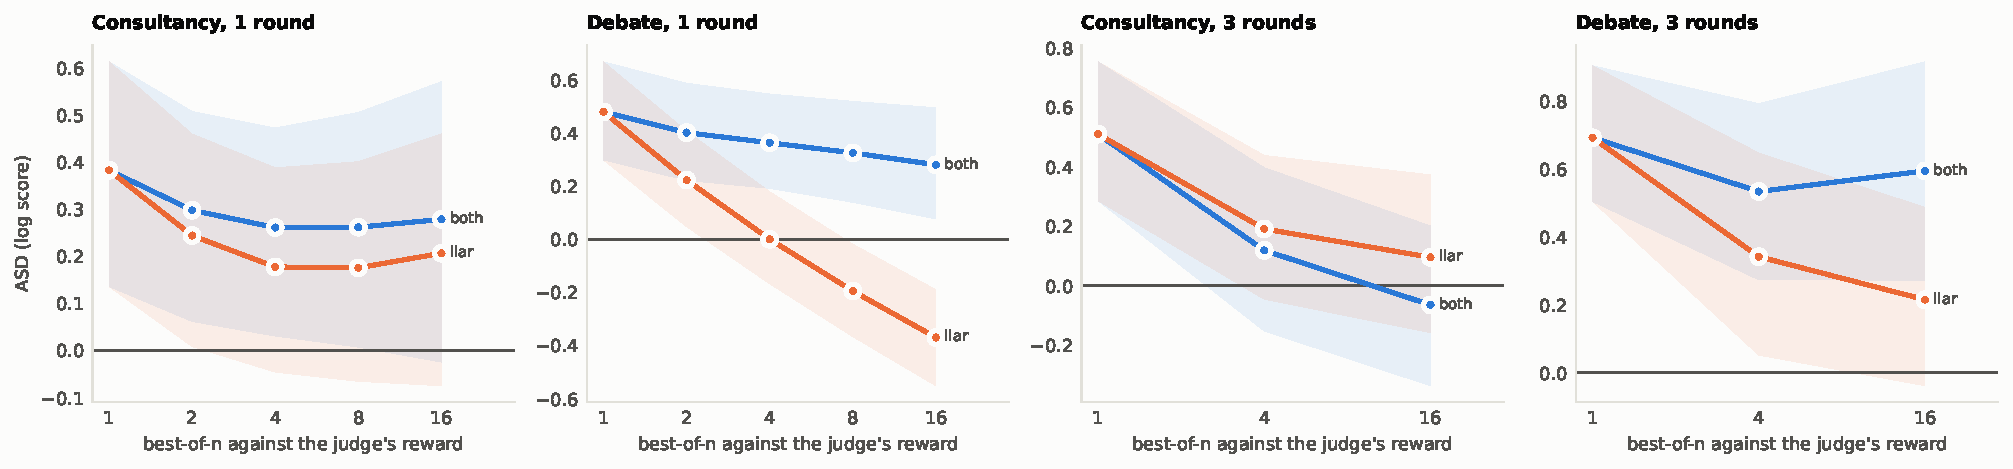
\includegraphics[width=\linewidth]{fig2_eic_under_best_of_n_paper.pdf}
\caption{EIC along best-of-$n$, held-out judging. Blue: both sides optimized; orange: only the liar.}
\label{fig:bon}
\end{figure}

Best-of-$n$ moves the agent along Eq.~\eqref{eq:cov}'s path, so the change of EIC with $n$ shows whether the
protocol stays incentive compatible as optimization proceeds (Figure~\ref{fig:bon}). In one round, optimizing only
the liar reverses debate's incentive: at best-of-16 the ASD is $-0.37$\ci{-0.55}{-0.19} and honesty wins on 29\% of
items. Optimizing both sides keeps it positive ($+0.28$\ci{+0.08}{+0.50}). With three rounds and best-of-16 on every
speech, debate keeps a positive incentive with both sides optimized ($+0.60$\ci{+0.27}{+0.92}), and with only
the liar optimized it falls to a third of its starting value ($+0.22$\ci{-0.04}{+0.49}); consultancy's falls to zero either way ($-0.06$ and
$+0.10$). Extra rounds let the honest debater rebut a better lie, which consultancy's judge cannot.

\begin{figure}[t]
\centering
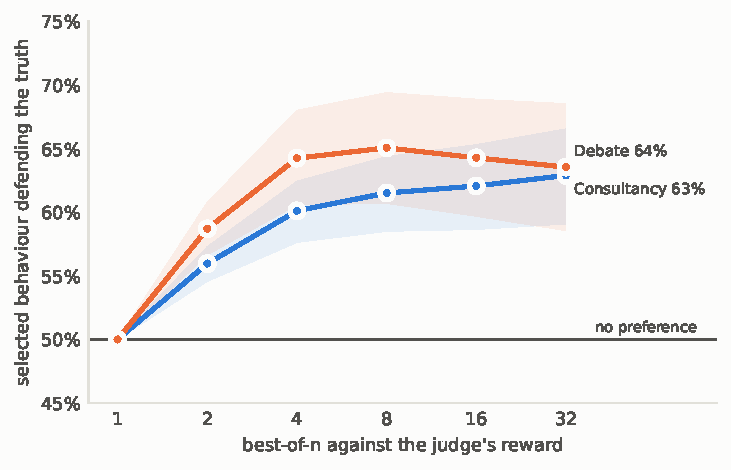
\includegraphics[width=0.55\linewidth]{fig4_choosing_a_side_paper.pdf}
\caption{An agent that chooses which answer to defend, optimized by best-of-$n$ over both sides' candidates: share
of its selected behaviour that is honest (one round, held-out).}
\label{fig:choice}
\end{figure}

When the agent may choose its side, best-of-$n$ selects honest behaviour more often: from 50\% to
62\%\ci{59}{65} (consultancy) and 64\%\ci{60}{69} (debate) at $n = 16$ (Figure~\ref{fig:choice}). The push toward
honesty is real but weak, and saturates by $n = 8$.

\section{Prompt optimization}\label{sec:po}

\begin{figure}[t]
\centering
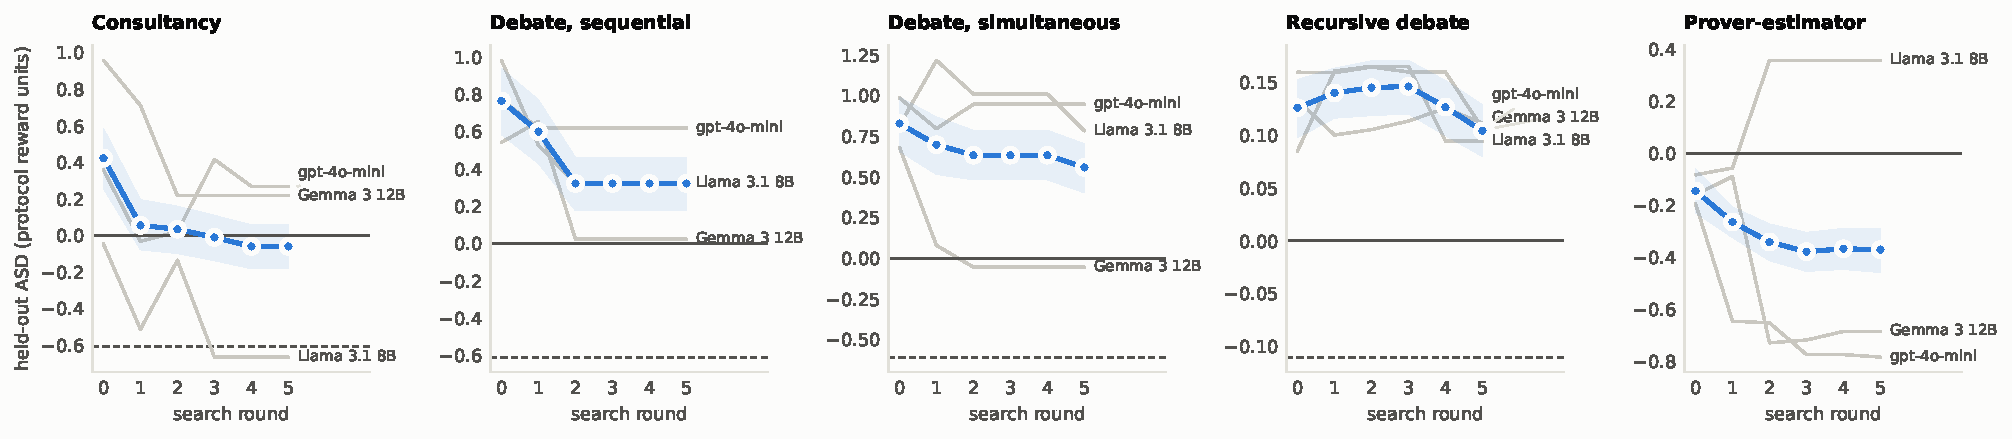
\includegraphics[width=\linewidth]{fig3_eic_prompt_optimization_paper.pdf}
\caption{EIC along prompt optimization: held-out ASD of the best honest vs best deceptive strategy after each search
round (gpt-5-mini; blue: judges pooled; gray: each judge).}
\label{fig:po}
\end{figure}

\begin{table}[t]
\centering\small
\caption{EIC under prompt optimization (held-out, 3 judges pooled): round 0 is the unprompted agent on each side;
round 5 the best strategies after five rounds of search.}
\label{tab:po}
\begin{tabular}{lccc}
\toprule
protocol & round 0 & round 5 & concordance, round 5 \\
\midrule
consultancy & $+0.55$ & $-0.24$\ci{-0.61}{+0.11} & 0.50 \\
debate, sequential & $+0.92$ & $+0.37$\ci{-0.04}{+0.75} & 0.69 \\
debate, simultaneous & $+1.10$ & $+0.69$\ci{+0.25}{+1.07} & 0.75 \\
recursive debate & $+0.13$ & $+0.09$\ci{+0.03}{+0.16} & 0.59 \\
prover-estimator & $-0.15$ & $-0.37$\ci{-0.46}{-0.29} & 0.16 \\
\bottomrule
\end{tabular}
\end{table}

Prompt optimization is the strongest sampler here (Figure~\ref{fig:po}, Table~\ref{tab:po}). Every protocol's EIC
falls as the searches proceed, because deception improves faster than honest argument. Consultancy's incentive is
erased: under Llama-3.1-8B and Gemma-3-12B the best deceptive consultant out-earns the best honest one on held-out
items. Prover-estimator's deficit deepens. Debate's EIC shrinks by 40--60\% but stays positive when pooled
over judges, significantly so for simultaneous debate; recursive debate's small positive incentive barely moves.
Over every strategy the searches produced (a population covariance rather than a frontier), the honest-minus-deceptive
reward is $+0.41$\ci{+0.11}{+0.72} for sequential debate, $+0.50$\ci{+0.16}{+0.84} for simultaneous debate and
$+0.16$\ci{-0.08}{+0.40} for consultancy.

\section{Do the samplers agree?}\label{sec:agreement}

\begin{figure}[t]
\centering
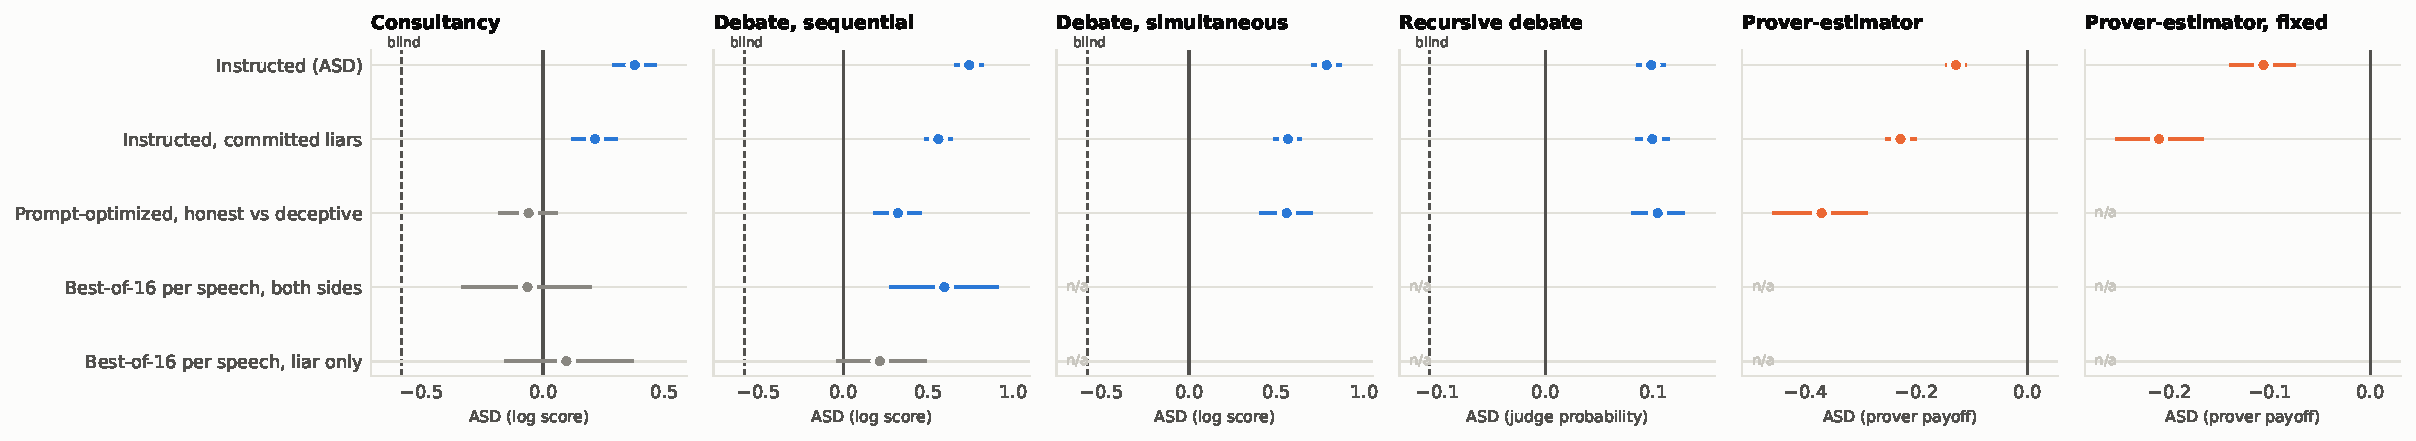
\includegraphics[width=\linewidth]{fig1_eic_by_sampler_paper.pdf}
\caption{EIC (ASD) of each protocol under each sampler, gpt-5-mini, judges pooled. Blue: interval above zero; orange:
below; gray: overlaps zero.}
\label{fig:headline}
\end{figure}

Figure~\ref{fig:headline} collects the samplers. The instructed sampler and its committed-liar variant rank the 15
(protocol, judge) cells almost identically (Spearman $0.99$), but either ranks them only loosely like prompt
optimization does ($0.40$ across cells; within a judge it ranges from $-0.21$ to $+0.80$;
Figure~\ref{fig:agree}). Instructed ASD gets the extremes right on average---prover-estimator is not incentive
compatible, debate is---but misses which protocols survive optimization under a given judge. Under Gemma-3-12B it
rates consultancy the most incentive-compatible protocol ($+0.91$\ci{+0.76}{+1.06}); against optimized deception
consultancy's EIC there is $-0.24$. Under Llama-3.1-8B, conversely, prover-estimator turns positive after
optimization ($+0.36$\ci{+0.21}{+0.50}) while every instructed estimate is negative.

\begin{figure}[t]
\centering
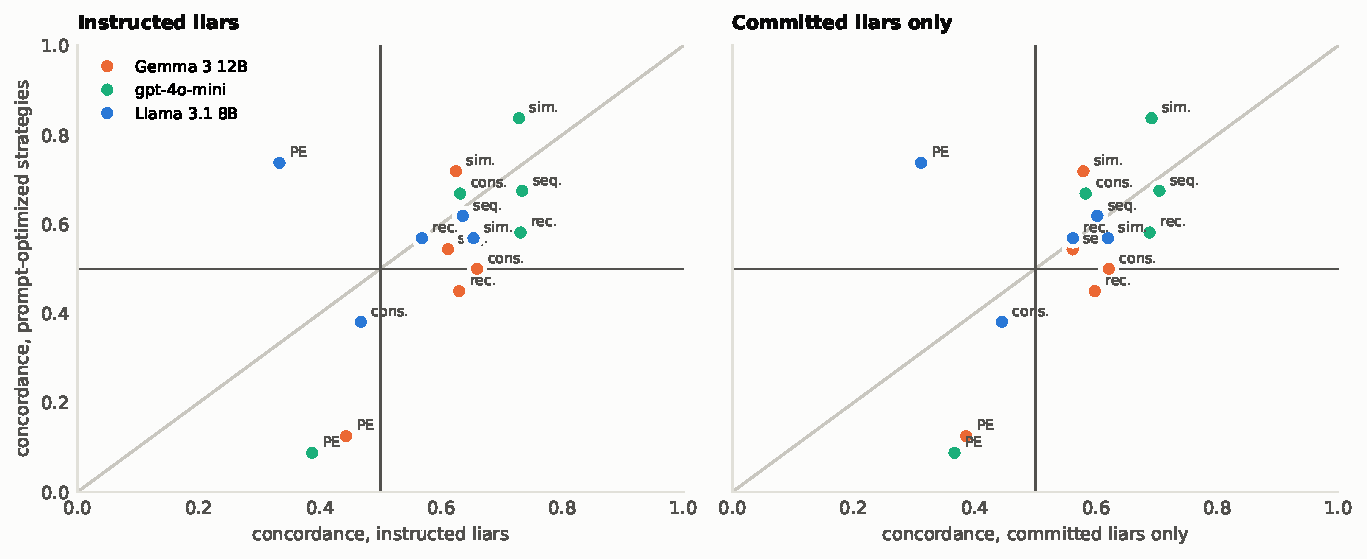
\includegraphics[width=0.85\linewidth]{fig8_sampler_agreement_paper.pdf}
\caption{Concordance under the instructed samplers vs prompt optimization, one point per (protocol, judge).}
\label{fig:agree}
\end{figure}

\section{EIC and judge capability}\label{sec:judges}

\begin{figure}[t]
\centering
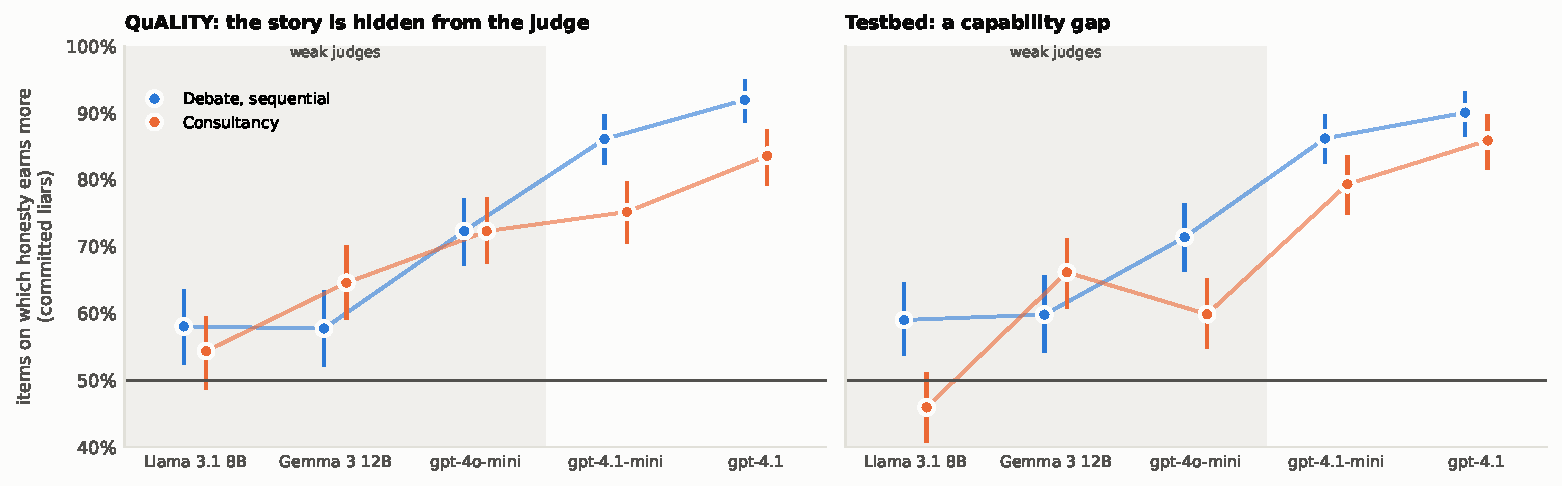
\includegraphics[width=\linewidth]{fig5_eic_by_judge_paper.pdf}
\caption{Concordance of the same debates and consultancies judged by five judges (committed liars).}
\label{fig:judges}
\end{figure}

Debate transcripts do not depend on the judge, so we re-judged every stored debate with two stronger judges
(gpt-4.1-mini, gpt-4.1), replaying the debaters' speeches exactly, on our testbed and on QuALITY
\citep{pang2022quality} (the story hidden from the judge). EIC rises steeply with judge capability
(Figure~\ref{fig:judges}): in debate, honesty wins on 58--61\% of items with Llama-3.1-8B and 90--92\% with gpt-4.1,
on both datasets. On the testbed the stronger judges already answer 87--90\% of items correctly alone, and
committed liars \emph{lower} their accuracy by 12--22 points, yet the protocols' incentive under them is the
highest we measured. Accuracy and incentive compatibility dissociate, as the argument for measuring incentives
predicts.

\section{Liars that refuse}\label{sec:tournament}

\begin{figure}[t]
\centering
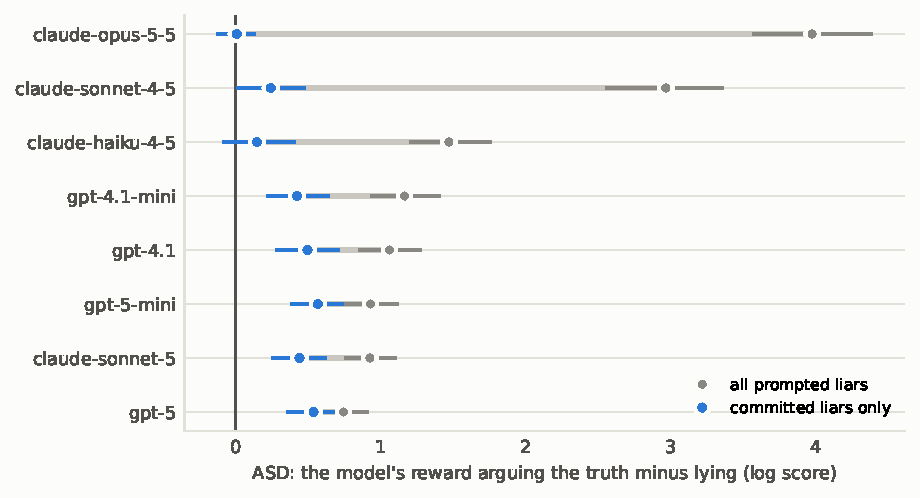
\includegraphics[width=0.66\linewidth]{fig6_tournament_paper.pdf}
\caption{Per debater model: reward arguing the truth minus lying, against every opponent in an 8-model debate
tournament (21{,}570 verdicts), all prompted liars vs committed liars only.}
\label{fig:tournament}
\end{figure}

In a tournament of eight debater models (Figure~\ref{fig:tournament}), the per-model EIC with prompted liars ranges
from $+0.74$ (gpt-5) to $+3.98$ (Claude Opus~5.5). The spread is almost entirely refusal: Opus~5.5 stays committed in
28\% of its lies (and refuses outright in 446 of 600 lying consultancies), gpt-5 in 98\%. With committed liars only,
every model's EIC lies between $0.0$ and $+0.6$. Instructed samplers built from safety-trained models overstate
incentive compatibility severely (Opus~5.5: $+3.98$ with all prompted liars, $+0.01$ with committed ones); the
effective-lie sampler or an optimizing sampler is needed.

\section{Hazards in measuring incentives against LLM judges}\label{sec:hazards}

\paragraph{Judge noise.} Two independent samples of the same judge on the same argument correlate $r = 0.08$--$0.33$
within an item. Any sampler that selects on one judge sample and scores on the same one inflates the effect of
optimization (in-sample best-of-16 consultancy liars appear to push the judge to 0.36 accuracy; held out, 0.55).
Covariance estimates are attenuated by the same noise.

\paragraph{Reward scale.} Log-score rewards grow with the judge's confidence, so ASD in log-score units is not
comparable across judges; concordance and $r$ are.

\paragraph{Last-word bias.} Weak judges side with the debater who speaks second: in sequential debate the honest side
wins 0.75 of the time speaking second and 0.42 speaking first. Seat balancing is necessary for any EIC estimate of
sequential protocols.

\section{Discussion}

The question for a training method is whether optimizing against it rewards honesty. On conceptual reasoning with
weak judges, the answer depends on the protocol and on the optimizer. Instructed liars make consultancy, debate and
recursive debate all look incentive compatible. A prompt optimizer that searches for good lies breaks consultancy and
leaves debate's incentive positive but diminished; prover-estimator debate without a trained estimator rewards lying
under every sampler. The incentive grows with the judge's capability, far more than with the protocol.

\paragraph{Limitations.} $v$ is by construction and binary; graded ground truth (e.g.\ expert-rated essays) would
allow richer behaviour spaces. The optimizers are inference-time; whether EIC under these samplers predicts the effect
of RL training is the open question this study prepares for but does not answer. The prompt-optimized liars were not
audited for commitment. Judges are LLMs, not people.

\paragraph{Reproducibility.} All experiments use the open-source \texttt{so-arena} library. The scripts are in its
\nolinkurl{experiments/} directory, the data and tables in \nolinkurl{docs/results/}. Total API spend was
about \$5{,}960.

\bibliographystyle{plainnat}
\bibliography{refs}

\appendix
\section{Judge accuracy (secondary)}
For completeness: with committed liars, consultancy, debate and recursive debate raise the weak judges' accuracy by
11--14 points over the judge alone (about a fifth of the 54-point gap), prover-estimator by 5. Under information
asymmetry (QuALITY) the weak judges gain 0--16 points from debate and the gpt-4.1 judges 25--27. Full tables are in
\nolinkurl{docs/results/decisive.md} and \nolinkurl{decisive_extended.md}.

\end{document}
